\chapter{\TitreChapitreDeux}\label{chap:Ceramique}

\bfigh
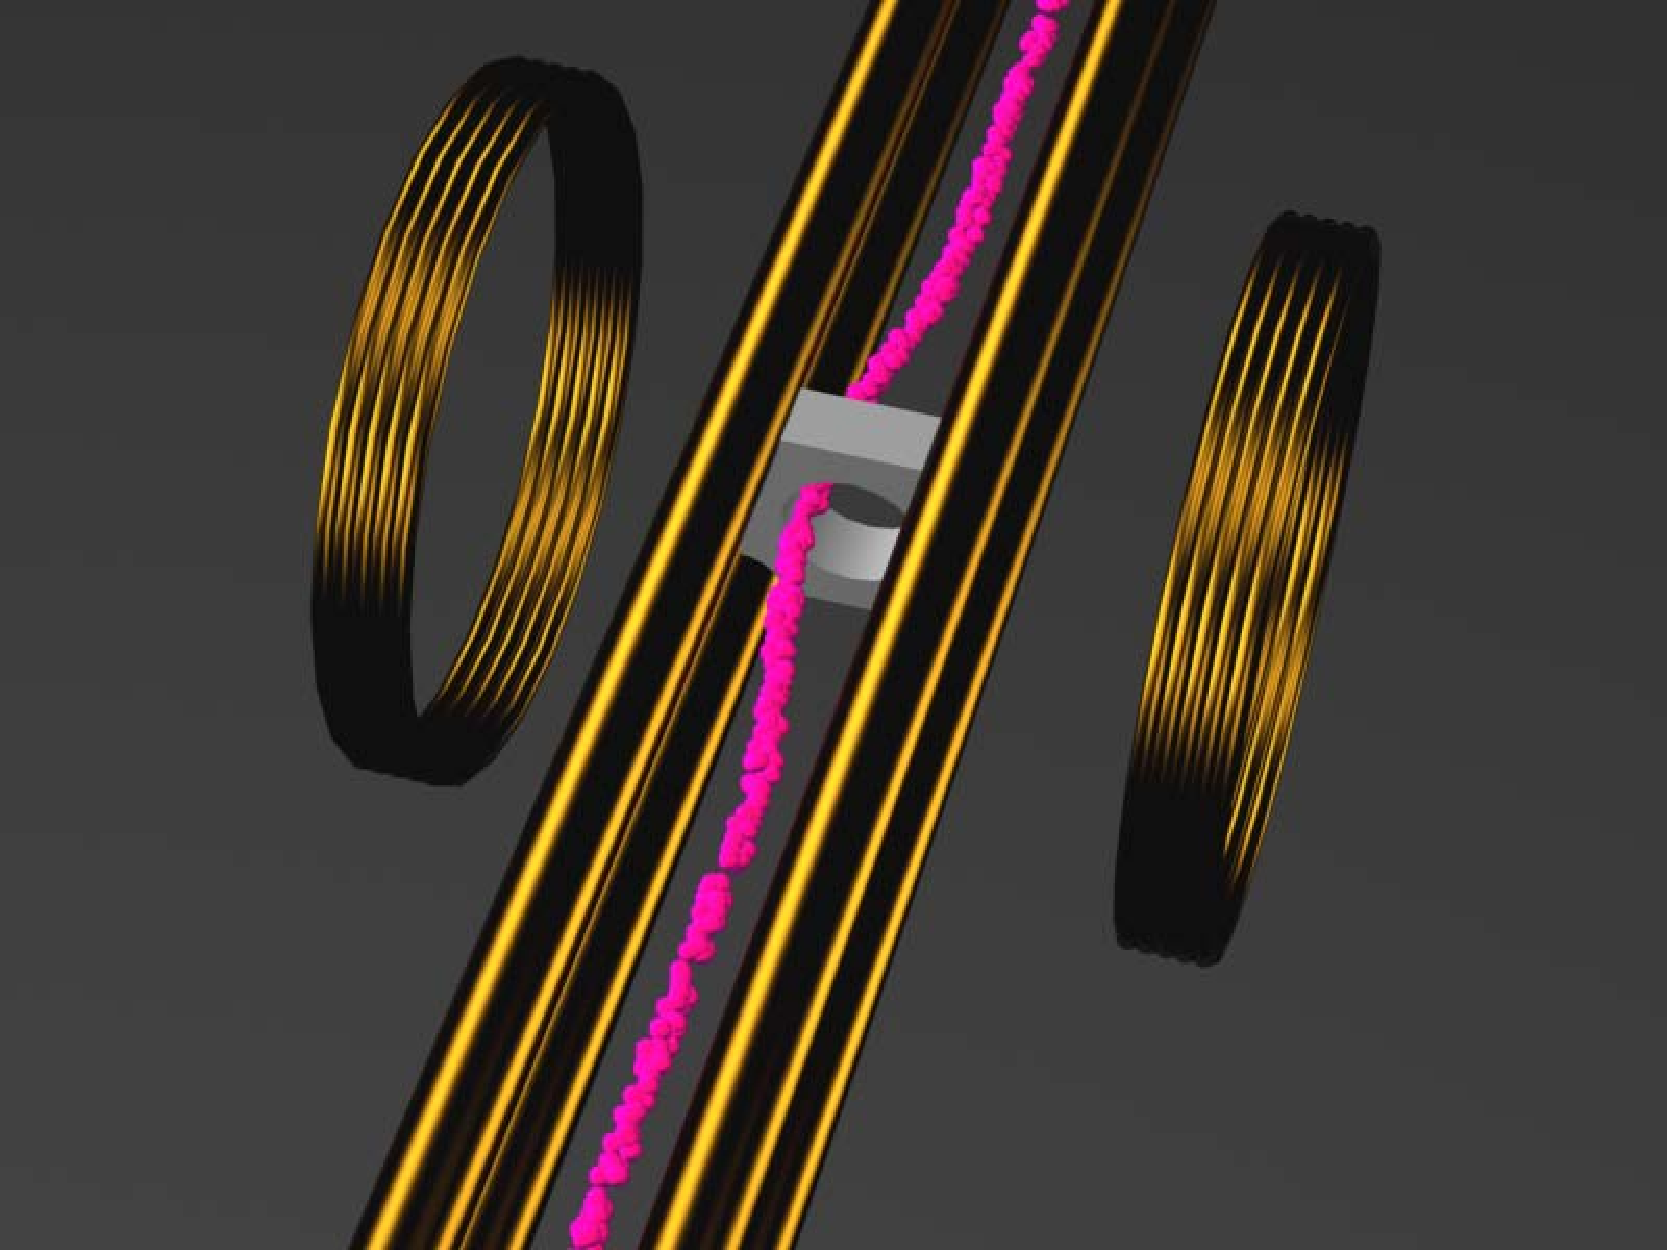
\includegraphics[width=\FigWidth]{P1/ChapitreCeramique}
\SansCaption
\efigh

\pagebreak

\minitoc
\vspace{0.5cm}
 
Dans le chapitre précédent, nous avons décrit le \setup qui nous permet d'effectuer l'\evap d'un \jatgm. Rappelons que le \fispse des atomes énergétiques y est mené à bien par la mise en place d'antennes radio-fréquences et micro-ondes le long du \gm. Cette technique usuelle d'évaporation souffre cependant d'un défaut majeur : si l'efficacité du filtrage est d'autant plus grande que la puissance de l'onde électromagnétique est élevée, la portée de l'antenne augmente alors également. Celle-ci est d'environ \cm{20} pour une antenne \rf utilisée dans les conditions expérimentales décrites dans la \autoref{sec:Gain10}. 

Dans la perspective d'utiliser un grand nombre de zones d'évaporation, il est primordial de pouvoir disposer d'une technique de \fisp \emph{efficace} et d'action \emph{très locale}. 
Dans ce chapitre, nous présentons une méthode qui répond à ces deux critères. Elle consiste en l'élimination sélective d'atomes par adsorption sur une surface diélectrique. 


\section{Mise en \oe uvre}\label{sec:EvapCeramMiseEnOeuvre}
L'évaporation par élimination d'atomes au contact d'une surface matérielle a été démontrée pour la première fois en 2003 par le groupe d'Eric Cornell~\cite{HMO03}. Ces travaux  montrent en outre que le caractère isolant (diélectrique) du matériau utilisé joue un rôle primordial : d'importantes pertes d'atomes sont observées lorsqu'un nuage magnétiquement piégé est approché à quelques dizaines de microns de la surface d'un conducteur%
\footnote{La raison en est que les fluctuations thermiques de courant à l'échelle microscopique d'un conducteur sont suffisantes pour induire de fortes fluctuations de \chm au voisinage de sa surface. Ces fluctuations peuvent alors provoquer des transitions entre \snZ vers des états non-piégés~\cite{HMO03,LTC04}.}%
.

\casse

Pour une surface en cuivre, excellent conducteur, les pertes commencent à se faire ressentir à une distance d'environ $\micron{200}$. 
En revanche, l'utilisation d'une surface de silicium permet de d'éliminer selectivement les atomes par contact avec la surface afin de mener à bien l'évaporation, éventuellement jusqu'au \rdq~\cite{LTC04}.


Cette section expose le principe de cette technique, ainsi que sa mise en \oe uvre sur notre \setup, \cad transposée au cas d'un \jatgm.


\subsection{Principe de la méthode}
Cette sous-section expose le principe de la méthode d'élimination d'atomes au contact d'une surface. Cette technique consiste en un \fispse d'atomes piégés par un champ de forces conservatives. 
Elle consiste 
%, comme dans le cas de l'évaporation par \firf, 
à éliminer les atomes dont l'énergie mécanique est élevée et sont la trajectoire atteint la surface d'un solide placé à proximité du piège. Au contact de celle-ci, les atomes sont éliminés%
\footnote
{
On peut raisonnablement considérer deux processus expliquant pourquoi l'atome qui entre en contact avec la surface est éliminé du piège:
\begin{itemize}
	\item l'adsorption, \cad que l'atome reste \sotosay{collé} à la surface et ne revient plus dans le piège.
	\item la surface étant à température ambiante ($\approx\SI{300}{\kelvin}$), l'agitation thermique de celle-ci peut communiquer une énergie cinétique considérable à toute particule qui  entre en contact avec elle. L'atome est alors \sotosay{éjecté} du piège.
\end{itemize}
}
du piège (voir la figure~\nref{fig:CeramPrincipe}).
\bfigh
\RemonteUnPeuFig
\subfloat[]
{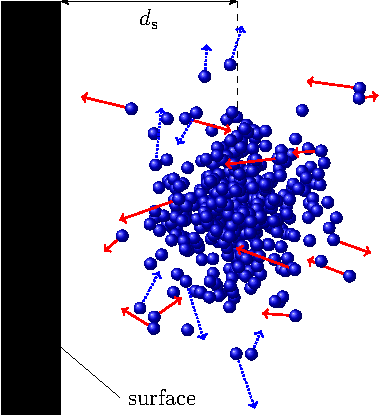
\includegraphics{P1/CeramPrincipe_a}} \qquad \qquad \qquad
\subfloat[]
{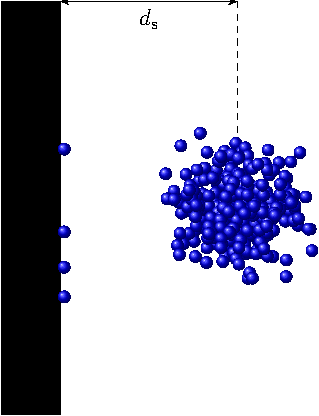
\includegraphics{P1/CeramPrincipe_b}}
\CaptionFigss{Principe de l'élimination sélective d'atomes sur une surface matérielle. \\
(a) : Un piège atomique est approché à une distance $\CeramDist$ d'une surface matérielle. Certains atomes (ceux dont le vecteur vitesse a été représenté) possèdent assez d'énergie mécanique pour atteindre la surface. Cependant, certains de ces atomes (dont le vecteur vitesse est représenté en pointillé) n'atteindrons pas la surface du fait de l'orientation de leur trajectoire. Ce mode d'évaporation est a priori unidimensionnel, \cad qu'il n'agit que sur un degré de liberté. \\
(b) : au contact de la surface, les atomes ont été éliminés du piège. Via les \colels entre atomes restants, le système évoluent vers un nouvel état d'\eqthdy d'énergie moyenne plus faible. Pour poursuivre l'évaporation, on peut alors diminuer à nouveau la distance $\CeramDist$.
}
\label{fig:CeramPrincipe}
\efigh

\subsection{Adaptation de la technique à un \jmg}
Afin d'adapter cette technique à un \jmg, il nous faut dévier la trajectoire de ce dernier vers une surface diélectrique placée dans le système à \uv. Notre \setup n'ayant initialement pas été prévu pour cette tâche, nous avons mis à profit les pièces de céramique qui servent à maintenir les tube de notre \gm (voir la figure~\nref{fig:CeramGuide}). 
\bfigh
\RemonteUnPeuFig
\subfloat[]
{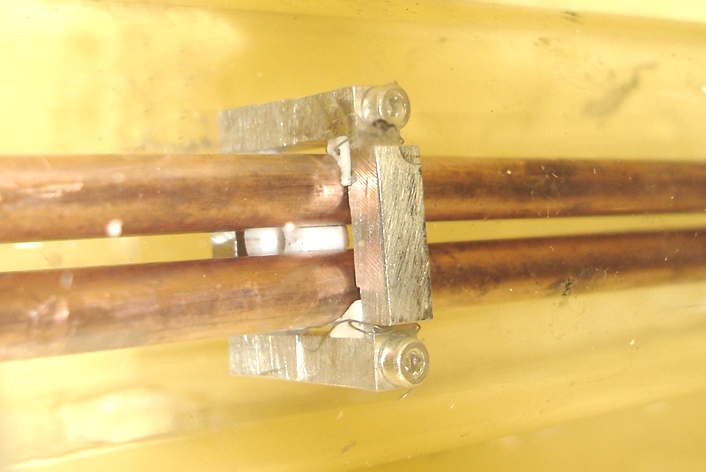
\includegraphics[height=6cm]{P1/DSC03881_Modif}}
\subfloat[]
{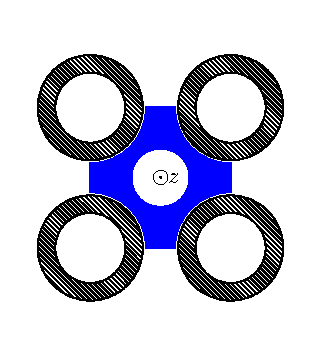
\includegraphics{P1/CeramTubes}} 

\RemonteUnPeuFig
\subfloat[]
{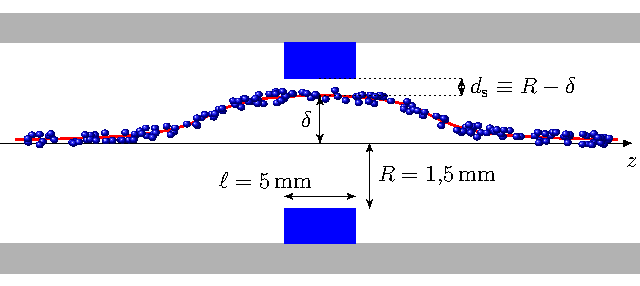
\includegraphics{P1/CeramTubesVueHaut}\label{fig:CeramGuide_c}}
\CaptionFig{Afin de maintenir les quatre tubes de cuivre à une distance donnée les uns des autres, des pièces de céramique sont réparties environ tous les \cm{40} le long du guide. La photographie (a) représente l'une de ces pièces à l'intérieur du tube de verre dans lequel règne un vide poussé. Le schéma (b) représente une coupe à l'échelle $3$ du guide au niveau d'une pièce de céramique (dessinée en bleu). La longueur d'une céramique est $\CeramLong=\mm{5}$. Le trou central de rayon $\CeramRay=\mm{1,5}$ permet au \jat de se propager suivant l'axe $z$ du guide. Le schéma (c) montre, vu de dessus, le jet localement dévié d'une distance $\Devi$ hors de cet axe. Si cette déviation se fait lors du passage dans l'une des céramiques, des atomes suffisamment énergétiques du jet peuvent être éliminés.}
\label{fig:CeramGuide}
\efigh

\ifthenelse{\FormatEUE > 0}{}
{\AjouteLigne}

Les \pdecs sont réparties environ tous les \cm{40} tout au long du guide et comportent un trou central de rayon $\CeramRay=\mm{1,5}$ %
\nome{\CeramRay}{Rayon du trou central des \pdecs}%
 au centre duquel passe le jet d'atome froids. L'extension longitudinale (selon l'axe $z$) de ces pièces est de $\CeramLong=\mm{5}$%
\nome{\CeramLong}{Extension longitudinale (selon l'axe $z$) des \pdecs}.
Il s'agit alors de dévier la trajectoire du jet d'une distance $\Devi$%
\nome{\Devi}{Déviation de la trajectoire du jet hors de l'axe $z$ du guide}%
 hors de l'axe $z$ vers le bord de l'une de ces \pdecs (voir la figure~\nref{fig:CeramGuide_c}). 


\subsubsection{Rappel sur le \gm}
Avant toute chose, rappelons que les quatre tubes de cuivre du guide produisent une configuration \qp de \chm.
Celle-ci se caractérise par une valeur minimale du champ tout au long de l'axe $z$ du guide. C'est autour de cette ligne que les atomes piégés dans l'état $\EtatFmF{1}{-1}$ orbitent durant leur propagation. 
Rappelons ici l'expression du vecteur \chm produit au voisinage de l'axe $z$ du guide (voir \vpageref{sec:ConfigMagnetiqueGuide}):
\[
	\vectBxyz = \vVecteur{-\gradB\,x}{\gradB\,y}{\Bpara} \mbox{\qquad avec \qquad} \gradB \equiv \frac{4\,\mu_0}{\pi\,\espTubes^2}\,I 
	\virguleformule
%	\label{eq:BQuadrAgain}
\]
où $\gradB\approx\gausspcm{800}$ est le \gtchm produit par le guide et $\Bpara\approx\gauss{1}$ est le champ uniforme longitudinal que nous ajoutons afin de minimiser les pertes par retournement de spin (voir \vpageref{AN:ValeurB0}).
\Remarque{
Dans tout ce chapitre, la température typique du \jat est de l'ordre de \microK{600}. Dans ces conditions, et comme nous l'avons vu dans la \autoref{sec:ConfigMagnetiqueGuide}, le \ppt \sotosay{ressenti} par les atomes est alors essentiellement linéaire (le paramètre $\alpha$ vaut environ $0,05$).%qui permet de mesurer l'harmonicité apparente du
}
La figure~\nref{fig:GuideChampTransverse_a} représente quelques lignes de champ dans un plan $(x,y)$, perpendiculaire à l'axe du guide. La figure~\nref{fig:GuideChampTransverse_b} montre, quant à elle, quelques vecteurs champs dans le plan horizontal $(x,z)$ contenant l'axe $z$ du guide. 
\bfigh
\subfloat[]
{\label{fig:GuideChampTransverse_a}
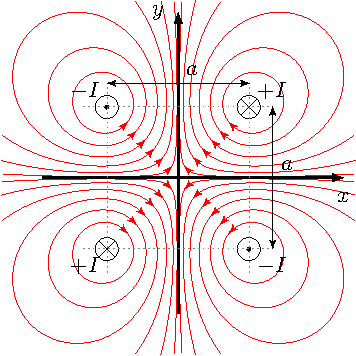
\includegraphics{P1/TubesQuadrupole_a}
}
\subfloat[]
{\label{fig:GuideChampTransverse_b}
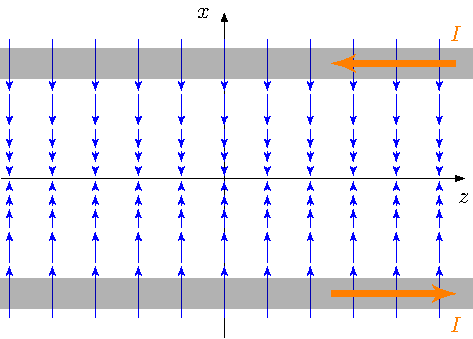
\includegraphics{P1/TubesQuadrupole_XZ}
}
\CaptionFig{Configuration de \chm \qpdd. (a): représentation de quelques lignes de champ dans le plan transverse $(x,y)$. (b) : dessin de quelques vecteurs champs dans une vue de dessus contenant l'axe du guide (l'unité de longueur des vecteurs est arbitraire). Le champ converge vers l'axe $z$ dans le plan $(x,z)$, et il diverge dans le plan vertical $(y,z)$. 
La position des tubes de cuivre est représentée par des zones grisées.}
\label{fig:GuideChampTransverse}
\efigh

\pagebreak

\subsection{Déviation du jet à l'aide d'une paire de bobines}\label{sec:EvapCeramBobines}
%Si nous pouvons utiliser l'une des \pdecs afin d'éliminer des atomes du jet, il nous faut encore disposer d'un moyen de dévier la trajectoire de ce dernier. 
Cette sous-section décrit l'une des deux méthodes que nous avons utilisées afin de dévier la trajectoire du jet. L'autre méthode (faisant intervenir des aimants permanents) fait l'objet de la \autoref{sec:EvapCeramAimants} en fin de ce chapitre.

Pour décaler la ligne qui correspond, à un minimum de module du \chm, il suffit de superposer localement un champ $\CeramBtrans$ %
\nome{\CeramBtrans}{Champ magnétique transverse permettant de dévier la trajectoire du jet}%
suivant une direction perpendiculaire à l'axe $z$. Dans notre cas, la direction du champ $\CeramBtrans$ est prise suivant l'axe $x$ de manière à dévier la trajectoire dans un plan horizontal%
%\footnote{De cette manière, nous évitons et à s'affranchir ainsi de variations d'altitude}%
.
L'amplitude $\Devi$ de la déviation hors de l'axe $z$ est alors donnée par :
\begin{equation}
	\Devi = \frac{\CeramBtrans}{\gradB}
\pointformule
\label{eq:Devi}
\end{equation}
Il faut cependant veiller à ne pas moduler la composante longitudinale du \chm (selon l'axe du guide). Nous verrons en effet dans le chapitre~\nref{chap:MiroirMobile} que cela aurait pour effet de produire une \bapot le long de l'axe du guide. 

Nous utilisons deux bobines de rayon \cm{4,5} et réalisées avec 107 tours de fil de cuivre de \mm{1,8} de diamètre. Comme le montre la figure~\nref{fig:GuideChampTransBobines}, elle sont placées symétriquement de part et d'autre du guide, à \cm{5} de l'axe $z$%
%\footnote{Les bobines  tube de verre dans lequel règne l'\uv ayant un }%
 et sont parcourues \emph{dans le même sens} par un courant ajustable de $0$ à \SI{40}{\ampere}. 
\bfigh
\subfloat[]
{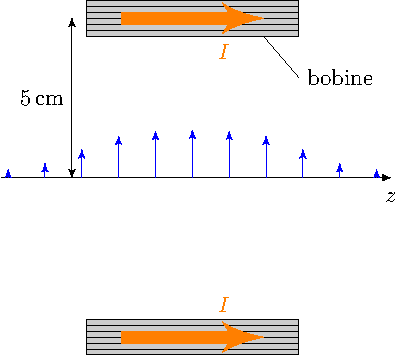
\includegraphics{P1/GuideChampTransBobines_a}
}
\subfloat[]
{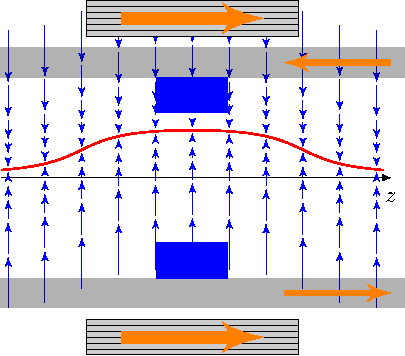
\includegraphics{P1/GuideChampTransBobines_b}
}
\CaptionFig{Représentation de l'effet de la superposition d'un \chm transverse sur le champ du guide.
(a) : dessins de quelques vecteurs champ pris le long de l'axe $z$, en ne considérant que les bobines positionnée symétriquement autour de l'axe du guide. 
(b) : représentation schématique de quelques vecteurs \chm lorsqu'on superpose le champ des bobines à celui du \gm. La ligne correspondant à un minimum local de \chm est déviée de l'axe $z$.}
\label{fig:GuideChampTransBobines}
\efigh

La configuration à deux bobines (qui rappelle une configuration Helmholtz) est parfaitement adaptée à nos besoins puisque le champ produit est purement transverse%
\footnote{Le champ est purement transverse sur l'axe $z$, mais ceci n'est plus vrai le long de la trajectoire moyenne des atomes qui est précisément déviée en dehors de cet axe. Cet effet est cependant complètement négligeable pour les extensions transverses considérées (voir l'application numérique).}
en tout point de l'axe $z$ du \gm. 
%De plus, le module du champ est quasiment constant au voisinage de la céramique. Ainsi le confinement transverse autour de la position d'équilibre n'est pratiquement pas modifié. 
\ApplicationNumerique{
Pour toutes les expériences décrites dans ce chapitre, le \gtchm fourni par le guide est égal à $\gradB=\gausspcm{800}$. Le champ transverse $\CeramBtrans$ créé au voisinage d'une céramique par la paire de bobines est proportionnel au courant qui les traverse et a été mesuré à \SI{9}{G\per\ampere}.

En terme de courant parcourant les bobines, l'amplitude $\Devi$ de la déviation du \jat est donnée par l'équation~\nref{eq:Devi} :
\[
\Devi = \frac{\CeramBtrans}{\gradB} \mbox{ , soit } \approx \SI{110}{\micro\meter\per\ampere}
\pointformule
\]
Le courant nécessaire pour dévier la trajectoire moyenne jusqu'au bord de la céramique (de rayon $\CeramRay=\mm{1.5}$) est de \SI{13}{\ampere}. 
}
Notons que même pour un tel courant, la composante longitudinale du champ le long de la trajectoire déviée reste très faible (inférieure à \SI{1}{G}). Nous verrons dans le chapitre~\nref{chap:MiroirMobile} que la colline de potentiel qui en résulte est donc complètement négligeable.
La situation aurait été singulièrement différente si une seule des deux bobines avait été utilisée pour dévier le jet (on atteindrait alors plusieurs dizaines de Gauss selon l'axe longitudinal).

\section{Résultats expérimentaux}
Dans cette section, nous présentons les résultats expérimentaux quant à l'effet d'une déviation de la trajectoire au niveau d'une \pdec. Ceci consiste principalement à étudier deux points :
\begin{itemizel}
	\item la réduction du \fat résultant directement du \fisp du jet,
	\item la variation de température du jet qui en résulte, après la \reth via les \colels entre atomes.
\end{itemizel}
\`A travers la mesure de ces deux grandeurs physiques, nous pourrons calculer les variations correspondantes de la \ddedpup. 


\subsection{Échauffement dû à la déviation du jet}
Dans la perspective d'utiliser notre technique pour le \rpef du jet, une étape préliminaire consiste à mesurer l'influence de la déviation du jet sur sa température. Le jet est en effet entrainé latéralement lors de son mouvement vers le bord de la céramique et les oscillations induites dans le \ppt peuvent induire un échauffement par un effet de \termetech{mélange non-linéaire}%
\footnote{Le mélange non-linéaire est illustré dans le chapitre~\nref{chap:PiegeDipolaire}, \vpageref{sec:MelangeNonLineaire}.}. 


\casse


Afin d'étudier ce point, nous installons les bobines dans une région du guide démunie de céramique. Ainsi, nous pouvons dévier le jet sans induire de pertes dues à la présence d'une surface. La température du jet est mesurée \m{3} en aval pour permettre une éventuelle \reth%
\footnote{La température du jet est mesurée par la technique décrite dans la section \vref{sec:MesureTempTrans}.}%
. 
En l'absence de déviation ($\Devi=0$) nous mesurons la température du jet à $T=\microKpm{630}{15}$. En présence d'une déviation importante, d'amplitude $\Devi=\mm{2}$, nous mesurons $T=\microKpm{620}{17}$. 
\Resultat
{
Il n'y a donc pas de chauffage notable dû à la déviation du \jat, tout du moins pour la gamme de températures dans laquelle nous travaillons.
}


\subsection{Variation du \fat}\label{sec:ResultatVariationFlux}
Revenons à l'étude du \fispse, avec les bobines placées au niveau d'une céramique. 
Nous nous intéressons dans cette sous-section à la variation du \fat induite par la déviation du jet vers la surface d'une \pdec. 
%
Nous comparons pour cela deux mesures de \fat%
\footnote{Nous utilisons la technique décrite dans la section \vref{sec:MesureDensiteGuideOuvert}.}%
:
\begin{itemize}
	\item une mesure du flux $\flux(\Devi)$ %
	\nome{\flux(\Devi)}{Flux atomique en aval de la céramique et en présence d'une déviation $\Devi$}%
	 en aval de la céramique et en présence d'une déviation d'amplitude $\Devi$,
	\item et une mesure du flux $\flux(\Devi=0)$ (toujours en aval de la céramique), mais en l'absence de déviation.
\end{itemize}
La figure~\nref{fig:CeramBobineFat} représente la fraction:%
\nome{\rapflux}{Rapport des \fats avec et sans déviation au niveau de la céramique}%
\[
\rapflux\equiv\frac{\flux(\Devi)}{\flux(0)}
\virguleformule
\]
en fonction de l'amplitude $\Devi$ de la déviation hors de l'axe $z$.
\bfighs
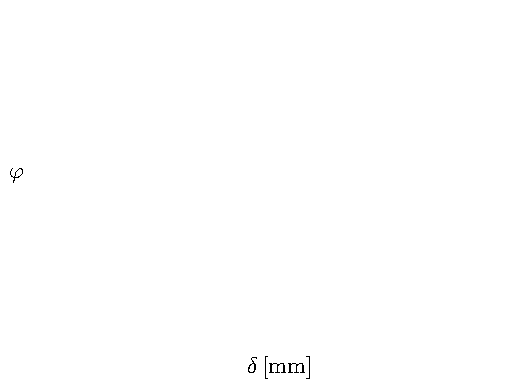
\includegraphics{P1/CeramBobineFat}
\CaptionFigs{Mesures représentant le rapport $\rapflux\equiv\ttfrac{\flux(\Devi)}{\flux(0)}$ des flux traversant la pièce en céramique avec et sans déviation, en fonction de l'amplitude $\Devi$ de la déviation hors de l'axe $z$ (selon l'axe $x$). Les valeurs négatives de $\Devi$ se rapportent à une déviation dans l'autre sens (vers les $x$ décroissants) et sont obtenues en changeant le sens du courant parcourant les bobines. On constate que si le jet est dévié de $\Devi\approx\CeramRay=\mm{1,5}$, tous les atomes sont éliminés.}
\label{fig:CeramBobineFat}
\efigh



\casse


\noindent Il est intéressant de discuter un point mis en évidence par la figure~\nref{fig:CeramBobineFat} : il apparait que la totalité des atomes sont éliminés sur la céramique si la trajectoire moyenne du jet est déviée de $\Devi\approx\CeramRay=\mm{1,5}$, \cad si celle-ci devient tangente à la surface. 
%
%\vspace{-0.6cm}


\subsubsection{Pouvions-nous prévoir ce résultat ?}
\inlinefig{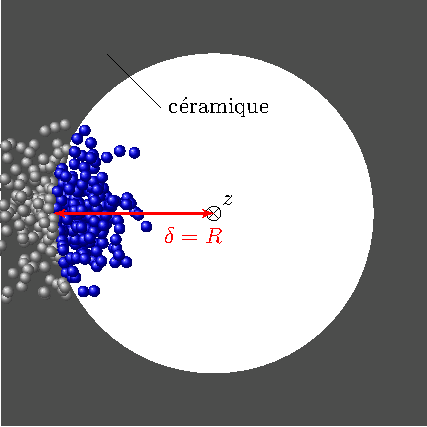
\includegraphics{P1/CeramAtomesDansCeram}} 
Dans le cas d'un nuage piégé, il semble évident que si le fond du piège est positionné au niveau de la surface ($\CeramDist~=~0$), tous les atomes vont y être éliminés après, au maximum, une demi-période d'oscillation. \label{Rq:PrevoirResultatDevi}

 Dans notre cas en revanche, le jet se propage suivant l'axe $z$ à une vitesse de \mps{1}. Ainsi, \emph{si la céramique était extrêmement fine} suivant l'axe $z$, seuls seraient éliminés les atomes qui se trouvent, au moment précis du passage dans la céramique, dans le demi-espace couvert par celle-ci. 
\noindent Sur le schéma ci-contre, qui représente une vue selon l'axe $z$, les atomes éliminés sont grisés. On s'attendrait donc à conserver environ la moitié des atomes (voir la figure \vref{fig:CeramBobineFatSimu}).
\picskip{0}
%\vspace{0.4cm}

\ApplicationNumerique
{
\noindent En réalité, la céramique possède une épaisseur $\CeramLong=\mm{5}$ suivant l'axe $z$. La vitesse moyenne du jet étant de $\vjet=\mps{1}$, chaque atome a besoin en moyenne d'un temps $\ttfrac{\CeramLong}{\vjet}=\ms{5}$ pour traverser la pièce de céramique. Ce temps est long devant la demi-période d'oscillation typiquement inférieure à \ms{0,5} (voir le chapitre~\nref{chap:JetAtomique}). C'est la raison pour laquelle tous les atomes sont éliminés pour une déviation d'amplitude $\Devi=\CeramRay=\mm{1,5}$.
}

\subsection{Gain en \ddedpup}\label{sec:ResultatVariationDDEDPUP}

Lorsqu'une partie des atomes les plus énergétiques du jet a été éliminée sur la \pdec, il s'en suit un retour vers un nouvel état d'\eqthdy%
\footnote{Nous avons en effet montré dans le chapitre~\nref{chap:JetAtomique} que le \jat que nous produisons possède un \tcolel suffisant pour autoriser la \reth.}%
.
Dans cette sous-section nous nous intéressons à la variation de température et de \ddedpup induite par le \fisp. 

\noindent Afin de mettre en évidence le refroidissement du jet, nous comparons toujours les résultats de deux mesures de température $T$, effectuées \m{3} en aval de la \pdec :
\begin{itemizel}
	\item une mesure $T(\Devi)$ correspondant au jet dévié d'une distance $\Devi$,
	\item et une mesure $T(\Devi=0)$ correspondant à la propagation habituelle du jet, \cad en l'absence de déviation. Dans notre cas, cette température est typiquement $T(0)=\microK{650}$.
\end{itemizel}



\Cahier{7,151}
\noindent Le tableau \vpageref[ci-dessous]{tab:CeramDDEDPUP} présente, pour différentes amplitudes $\Devi$ de déviation, quelques mesures expérimentales de rapports de températures 
$
\ttfrac{T(\Devi)}{T(0)}
%\virguleformule
$,
ainsi que les rapports de \fats
$
\rapflux=\ttfrac{\flux(\Devi)}{\flux(0)}
%\virguleformule
$
qui y sont associés. 

\noindent Ces deux données nous permettent de calculer%
\footnote{voir l'équation \vref{eq:rhojetaxe}.}
les gains correspondants pour la \ddedpup :
\[
%\GainDevi \equiv 
\frac{\rhojetaxe(\Devi)}{\rhojetaxe(0)}
\virguleformule
\]
où $\rhojetaxe$ désigne la \ddedpup sur l'axe du \jat:
\[
\setlength{\extrarowheight}{9 pt}\label{tab:CeramDDEDPUP}
\begin{array}{|c|c|c|c|c|}
\hline
   \Devi & 
   \mm{0,68} & \mm{0,79} & \mm{0,90} & \mm{1,0} \\
\hline
   \rapflux\equiv\frac{\flux(\Devi)}{\flux(0)} & 
   \val{0,88} & \val{0,82} & \val{0,71} & \val{0,60} \\
\hline
   \,\,\, \frac{T(\Devi)}{T(0)} \mbox{ avec } T(0)\approx\microK{650} \,\,\, & 
   \val{0,94}\pm\val{0,03} & \val{0,92}\pm\val{0,03} & \val{0,83}\pm\val{0,03} & \val{0,77}\pm\val{0,03} \\
\hline
   \frac{\rhojetaxe(\Devi)}{\rhojetaxe(0)} & 
   \val{1,08}\pm\val{0,09} & \val{1,09}\pm\val{0,09} & \val{1,34}\pm\val{0,11} & \val{1,50}\pm\val{0,12} \\
\hline
\end{array}
\]
\Resultat
{
%En utilisant une déviation de $\Devi=\mm{1,0}$ la température du jet obtenue après \reth est $T'=\microKpm{500}{10}$. La variation de \fat correspondant étant de $\rapflux=0,6$, nous
Nous pouvons donc obtenir un gain d'un facteur \val{1,5} en \ddedpup. Ceci s'accompagne d'une perte d'environ $10\%$ sur le \tcolel (voir la \autoref{sec:CeramSimuGainTcol}). Cette technique d'évaporation présente donc des performances comparables à l'évaporation par \firf décrite dans la \autoref{sec:EvapRf}.
}



\section{Dimensionnalité de l'évaporation}\label{sec:CeramBiDimensionnalité}
Comme nous l'avons mentionné dans la \autoref{sec:EvapCeramMiseEnOeuvre}, le processus d'évaporation par élimination sur une surface matérielle possède un caractère \emph{unidimensionnel}~\cite{HMO03} puisqu'il n'élimine les atomes qu'en fonction de l'un de leurs degrés de liberté en position%
\footnote{En toute rigueur, sur notre \setup, la surface interne de la céramique n'agit pas que sur un seul degré de liberté (suivant l'axe $x$). En effet, celle-ci n'est pas une surface plane~\cite{HMO03}, mais cylindrique. Elle agit donc aussi sur l'autre degré de liberté transverse (suivant l'axe $y$ dans notre cas).}
(suivant l'axe $x$ dans notre cas). 
On peut donc s'interroger sur son efficacité en terme de gain en \ddedpup. Nous pouvons en effet montrer que si l'évaporation concernait les deux degrés de liberté transverses, nous pourrions espérer un gain d'un facteur \val{3.4}~\cite{LaG05}.
%
Cette section a pour but de montrer pourquoi cette technique d'évaporation peu en fait aisément être rendue \emph{bidimensionnelle}.

\subsubsection{Redistribution de l'énergie mécanique transverse dans le \ppthyp}
Rappelons que le \ppt dans le \gm \emph{n'est pas de forme harmonique}, mais hyperbolique (voir la \autoref{sec:ConfigMagnetiqueGuide}). Le couplage entre les degrés de liberté transverses qui en résulte implique que les trajectoires atomiques projetées sur le plan transverse $(x,y)$ ne sont a priori pas des trajectoires fermées. La figure~\nref{fig:CeramTrajGuide_a} montre un exemple typique de trajectoire. On y voit bien la redistribution de l'énergie mécanique transverse suivant différentes directions du plan $(x,y)$ du fait que la trajectoire \sotosay{pivote}.

La figure~\nref{fig:CeramTrajGuide_b} montre d'ailleurs qu'une trajectoire atomique, qui n'atteindrait a priori pas la surface au moment où l'atome arrive au niveau de la céramique, peut en fait après un certain temps pivoter suffisamment pour l'atteindre.
%
\bfighss
\subfloat[]
{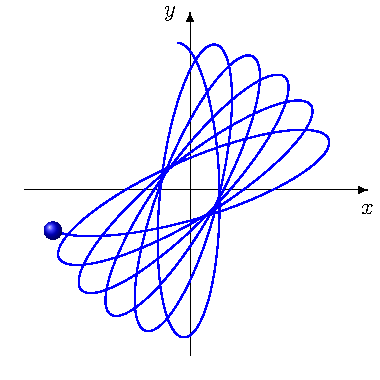
\includegraphics{P1/CeramTrajGuide_a}\label{fig:CeramTrajGuide_a}} \;
\subfloat[]
{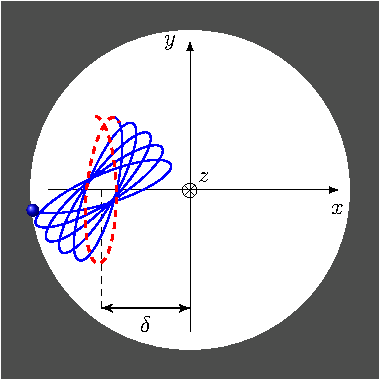
\includegraphics{P1/CeramTrajGuide_b}\label{fig:CeramTrajGuide_b}}
\CaptionFigs{Représentation d'une trajectoire atomique typique projetée dans le plan $(x,y)$. \\
(a) : Le \ppt non-harmonique fourni par le guide implique un couplage des degrés de liberté transverses. Ainsi, la direction pour laquelle l'atome est à l'apogée de sa trajectoire pivote au fil du temps. \\
(b) : Lorsqu'un atome pénètre dans le trou de la \pdec, sa trajectoire peut initialement ne pas atteindre la surface (partie rouge tiretée de la trajectoire). En effet, son énergie mécanique est essentiellement répartie selon la direction $y$. Cependant, au fil des oscillations, la trajectoire pivote et peut finir par atteindre la surface.% L'énergie mécanique est re-distribuée sur différente direction du plan ($x,y$).
}
\label{fig:CeramTrajGuide}
\efigh

\ifthenelse{\FormatEUE > 0}{}
{\AjouteLigne}
%
C'est cette redistribution au fil du temps de l'énergie mécanique sur différentes directions du plan $(x,y)$ qui peut rendre le processus d'évaporation presque aussi efficace que s'il était bidimensionnel. Il faut pour cela que les atomes restent suffisamment longtemps au niveau de la \pdec.
\Resultat
{
La \emph{dimensionnalité effective} de l'évaporation dépend de la longueur $\CeramLong$ de la \pdec suivant l'axe $z$ et de la vitesse moyenne $\vjet$ du \jat.
Pour nos paramètres expérimentaux typiques, une simulation numérique montre que l'évaporation serait considérée comme étant bidimensionnelle si la pièce de céramique avait une longueur d'au moins $\CeramLong=\cm{5}$ (voir la \autoref{sec:CeramSimuGain}).
}

\Remarque{Il convient de garder à l'esprit que la redistribution de l'énergie mécanique sur les degrés de liberté transverses est directement liée à l'anharmonicité du \ppt. Dans le cas d'un piégeage harmonique, les trajectoires sont toujours fermées, de forme elliptique.
Nous avons montré dans la \autoref{sec:ConfigMagnetiqueGuide} que la forme du potentiel auquel sont soumis les atomes dépend du facteur $\alpha$ défini à la \vpageref{Rq:alpha}.
% :
%%$\alpha = \ttfrac{\mu\,\Bpara}{\kb\,T}$ 
%\[
%\alpha = \alphaexpr
%\pointformule
%\]
Ainsi dans la perspective d'abaisser de plus en plus la température ($\alpha \ll 1$), nous finirons toujours par atteindre la limite d'un potentiel harmonique, et donc par annuler l'effet de bidimensionnalité décrit dans cette section.
}


\casse


\section{Interprétation des résultats}

Afin d'interpréter les variations de \fat en terme de \fispse, il serait utile de disposer d'une modélisation du problème. Cependant, dans le cas de l'évaporation du jet sur nos \pdecs, la formalisation du problème ne permet pas d'obtenir des résultats analytiques simples, et ce pour plusieurs raisons:
\begin{itemizel}
	\item le problème ne possède pas de symétrie de révolution autour de l'axe $z$ (contrairement au cas dans la \autoref{sec:MesureTempTrans} pour le \firf).
	\item Le \ppt n'est pas harmonique (voir la \autoref{sec:ConfigMagnetiqueGuide}). Comme nous l'avons vu, il en résulte un couplage entre les degrés de liberté transverses qui fait intervenir le temps passé au voisinage de la \pdec.
	\item la surface interne de la céramique n'est pas plane, mais cylindrique. Le critère de filtrage fait donc lui aussi intervenir les deux degrés de liberté transverses.
\end{itemizel}
Cette section a pour but de comparer nos résultats expérimentaux avec ceux obtenus grâce à des simulations numériques. Nous commençons, dans la sous-section suivante par décrire les \emph{ingrédients physiques} utilisés dans ces simulations.

\subsection{Simulations numériques}\label{sec:CeramSimu}
Les simulations numériques ont été effectuées par Antoine Couvert dans le cadre de son stage de DEA. La programmation en langage \termetech{Fortran 95}, met en \oe uvre une méthode de \termetech{Monte-Carlo} associée à un algorithme symplectique d'ordre~4~\cite{Yos93} pour calculer la trajectoire des atomes. 
Mentionnons que la simulation \emph{ne tient pas compte des \colels entre atomes}. Nous justifions cette simplification par le fait que les atomes restent au voisinage de la \pdec pendant typiquement \ms{5} (voir \vpageref{Rq:PrevoirResultatDevi}), alors que le \tcolel par atome est seulement de l'ordre de $\SI{10}{\reciprocal\second}$.
% \ll \ttfrac{1}{\val{0.005}}=\SI{200}{\reciprocal\second}$.

\noindent Les positions et vitesses initiales des atomes sont tirées aléatoirement par la méthode de réjection~\cite{PTV92} de manière à reproduire les grandeurs physiques qui caractérisent notre \jat, et que nous déterminons expérimentalement:
\begin{itemizel}
	\item la vitesse moyenne du jet $\vjet=\mps{1,0}$,
	\item sa température d'\eqthdy $T=\microK{650}$,
	\item le \gtchm imposé par le guide $\gradB=\gausspcm{800}$,
	\item le champ longitudinal $\Bpara=\gauss{1}$,
	\item la géométrie de la surface cylindrique de rayon $\CeramRay=\mm{1,5}$ et de longueur $\CeramLong=\mm{5}$.
\end{itemizel}
Pour reproduire le critère de \fispse, nous supposons que le jet se propage suivant une ligne droite (l'axe $z$), et qu'il passe au travers d'une \pdec qui, elle, est désaxée latéralement d'une distance $\Devi$. 
Nous supposons une \emph{efficacité d'évaporation de $100\%$}. Ainsi, toute trajectoire atteignant la surface du cylindre de rayon $\CeramRay=\mm{1,5}$, de longueur $\CeramLong=\mm{5}$ et dont l'axe est excentré d'une distance $\Devi$ par rapport à la trajectoire moyenne du jet, est considérée comme étant éliminée.


\casse


\subsection{Variation du \fat}

La figure~\nref{fig:CeramBobineFatSimu} représente les données expérimentales de la figure~\nref{fig:CeramBobineFat} (page \pageref{fig:CeramBobineFat}) ainsi que le calcul de $\rapflux$ obtenu par la simulation numérique. 
\bfighs
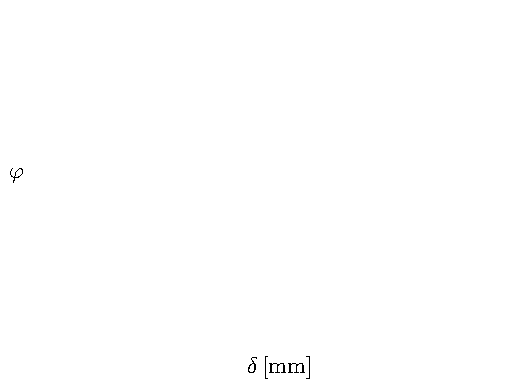
\includegraphics{P1/CeramBobineFatSimu}
\CaptionFigss{Représentation des variations du \fat en fonction de l'amplitude $\Devi$ de la déviation. Les données expérimentales de la figure~\nref{fig:CeramBobineFat} (page \pageref{fig:CeramBobineFat}) sont représentées par des carrés grisés. Les résultats de la simulation pour la fraction $\rapflux \equiv \ttfrac{\flux(\Devi)}{\flux(0)}$ sont représentés par une ligne continue. 
%Toutes les grandeurs physiques qui caractérisent le jet, le confinement et la géométrie de la pièce de céramique sont entrées dans la simulation telles qu'elles sont mesurées expérimentalement. Le seul ajustement effectuer sur le résultat de la simulation est un déplacement global de la courbe de \micron{-40} sur l'axe des abscisses. Ceci traduit simplement le fait que le trou central de la pièce de céramique utilisée est très légèrement désaxée par rapport à l'axe $z$.\\
La ligne pointillée représente le résultat de la simulation pour $\rapflux$ mais en considérant le cas d'une pièce de céramique de \emph{longueur extrêmement faible} ($\CeramLong=\micron{10}$). Dans ces conditions, comme nous l'avons mentionné dans la \autoref{sec:ResultatVariationFlux}, les atomes n'ont pas le temps d'effectuer une demi-période d'oscillation lors de la traversée de la céramique. On constate d'ailleurs, comme prévu dans ce cas, que pour une déviation d'amplitude $\Devi=\CeramRay=\mm{1,5}$, environ la moitié des atomes sont éliminés.
}
\label{fig:CeramBobineFatSimu}
\efigh


%\Remarque
{\label{Rq:DeviZero}
Rappelons que $\rapflux\equiv\ttfrac{\flux(\Devi)}{\flux(0)}$ est le rapport du flux traversant la céramique en présence d'une déviation $\Devi$ par le flux en l'absence de déviation ($\Devi=0$). 
Il est en effet important de ne pas confondre les deux grandeurs suivantes :
\begin{itemize}
	\item le flux \emph{traversant la céramique en l'absence de déviation} 
	\item et le flux \emph{en l'absence pur et simple de céramique}. 
\end{itemize}
%La deuxième de ces grandeurs n'est pas expérimentalement mesurable puisque les céramiques sont dans l'enceinte à vide. 
}
En outre, la simulation numérique montre que, \emph{même en l'absence de déviation}, le \fat est réduit d'environ $4\%$.
Ceci est dû au fait que, dans la gamme de température dans laquelle nous nous trouvons ($\approx\microK{650}$), la pièce de céramique élimine les atomes qui sont suffisamment énergétiques pour que leurs trajectoires s'éloignent de plus de $\CeramRay=\mm{1,5}$ de l'axe du guide. On s'attend à voir disparaître cet effet lorsque la température du jet est plus faible.
%\Resultat
%{}

Au vu de l'excellent accord avec les données expérimentales, il est important de rappeler que toutes les grandeurs physiques utilisées dans la simulation ont été mesurées expérimentalement. Il n'y a donc aucun paramètre ajustable, si ce n'est l'efficacité d'évaporation, que nous avons supposée de $\val{100}\%$.

\Remarque{
En fait, le seul ajustement effectué sur le résultat de la simulation correspond à déplacer globalement la courbe de la figure~\nref{fig:CeramBobineFatSimu} sur l'axe des abscisses. Ceci rend compte d'un léger parallaxe entre le trou central de la céramique et l'axe $z$.
Nous avons ainsi constaté que la pièce en céramique que nous utilisons pour nos expériences possède un trou désaxé de \micron{40} par rapport à l'axe du \gm.
}

\ifthenelse{\FormatEUE > 0}{}
{\AjouteLigne \AjouteLigne}

\subsection{Gain en \ddedpup}\label{sec:CeramSimuGain}
Intéressons nous maintenant à l'évolution des caractéristiques du jet après la traversée de la \pdec. La simulation ne tient pas compte des \colels entre atomes, qui sont indispensables pour accéder à la dynamique de la \reth. 
Nous pouvons néanmoins supposer qu'après le \fisp, le jet atteint un nouvel état d'\eqthdy, et effectuer un simple bilan d'énergie afin de déduire le gain $\GainCeram$ en \ddedpup:
%\RemonteUnPeuFig
\[
%\Delta\rhojetaxe \equiv 
\GainCeram \equiv \frac{\AvecTexte{\rhojetaxe}{après}}{\AvecTexte{\rhojetaxe}{avant}}
\virguleformule
\]
où $\AvecTexte{\rhojetaxe}{avant}$ et $\AvecTexte{\rhojetaxe}{après}$ sont les \ddedpup sur l'axe du jet, respectivement avant traversée de la céramique et après traversée de la céramique suivie d'une \reth.
% (voir la \autoref{sec:RethermJet}). 

La simulation permet de nous intéresser à des situations pour lesquelles la longueur $\CeramLong$ de la céramique serait différente de \mm{5}. 
La figure~\nref{fig:CeramBobineDDEDPUPSimu} représente les gains $\GainCeram$ en \ddedpup obtenus après \reth, et en considérant $\CeramLong=\micron{10}$, $\CeramLong=\mm{5}$, $\CeramLong=\mm{10}$ et $\CeramLong=\mm{100}$.
%
\bfighs
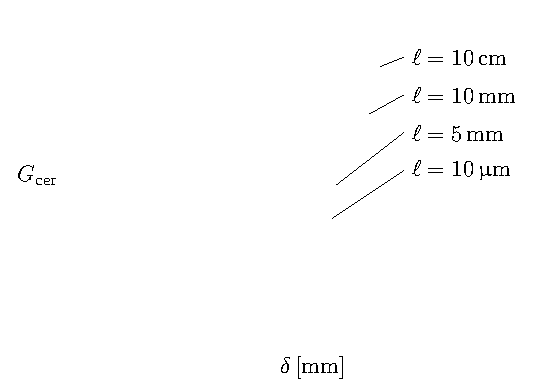
\includegraphics{P1/CeramBobineDDEDPUPSimu}
\RemonteUnPeuFig
\RemonteUnPeuFig
\CaptionTocCaptionFig{Représentation des résultats de la simulation numérique pour le gain en \ddedpup }{Représentation des résultats de la simulation numérique pour le gain en \ddedpup $\GainCeram%\equiv \ttfrac{\AvecTexte{\rhojetaxe}{après}}{\AvecTexte{\rhojetaxe}{avant}}
$ en fonction de la distance $\Devi$ de déviation. Les différentes courbes correspondent à différentes longueurs de la \pdec. On voit bien le caractère bidimensionnel de l'évaporation qui se manifeste avec l'augmentation de la longueur $\CeramLong$, comme mentionné en \autoref{sec:CeramBiDimensionnalité} (la ligne pointillée correspond précisément à une évaporation bidimensionnelle parfaite).
%Les symboles carrés correspondent à des données mesurées expérimentalement et sont donc à comparer à la courbe $\CeramLong=\mm{5}$.
}
\label{fig:CeramBobineDDEDPUPSimu}
\efigh

\casse

\subsubsection{Interprétation des résultats de la simulation numérique}\label{sec:CeramBobineDDEDPUPSimuInterpretation}
\noindent Proposons nous d'interpréter les résultats de la simulation présentés sur la figure~\nref{fig:CeramBobineDDEDPUPSimu}. On peut noter plusieurs points mis en évidence sur cette figure :
\begin{ditemize}
	\item comme prévu (voir la \autoref{sec:CeramBiDimensionnalité}), le caractère bidimensionnel de l'évaporation se manifeste lorsque nous prenons des longueurs $\CeramLong$ de plus en plus élevées. Pour $\CeramLong=\cm{10}$, on atteint quasiment les performances d'un processus d'évaporation à deux dimensions (ligne pointillée de la figure~\nref{fig:CeramBobineDDEDPUPSimu}).
	\item on constate que, \emph{même en l'absence de déviation} ($\Devi=0$), la \ddedpup du jet augmente sensiblement ($\approx+15\%$) du fait du passage dans la pièce de céramique. Ceci est la conséquence, comme nous l'avons noté dans la remarque \vpageref[ci-dessus]{Rq:DeviZero}, de l'élimination d'atomes suffisamment énergétiques pour qu'ils s'éloignent de plus de $\CeramRay=\mm{1,5}$ de l'axe $z$ du guide (le \fat est réduit d'environ $4\%$). 
	\item toutes les courbes (sauf pour $\CeramLong=\micron{10}$) convergent, quand $\Devi\rightarrow0$, vers la même valeur ($\approx\val{1.15}$) qui correspond aussi à celle obtenue pour une évaporation parfaitement bidimensionnelle. Ceci est prévisible dans la mesure où, si $\Devi=0$, la description du problème possède une symétrie de révolution. Le critère de \fisp et donc l'évaporation sont donc nécessairement bidimensionnels.
	\item la courbe correspondant à $\CeramLong=\micron{10}$ ne converge pas vers la même valeur que les autre quand $\Devi\rightarrow0$. En effet, comme nous l'avons vu dans la \autoref{sec:ResultatVariationFlux}, \emph{si la céramique est extrêmement fine}, les atomes n'ont pas le temps d'effectuer une demi-période d'oscillation au moment du passage dans celle-ci. N'est alors éliminé qu'une partie des atomes énergétiques qui devraient l'être.
	\item ce dernier point est d'ailleurs souligné par le fait qu'en $\Devi=\CeramRay=\mm{1,5}$, la totalité des atomes semblent être éliminés pour $\CeramLong \geqslant \mm{5}$, mais pas pour $\CeramLong=\micron{10}$ (voir \vpageref{Rq:PrevoirResultatDevi}).
\end{ditemize}



\subsubsection{Comparaison aux résultats expérimentaux}

Nous allons comparer les données de la simulation numérique aux résultats expérimentaux de la \autoref{sec:ResultatVariationDDEDPUP}. Il faut pour cela tenir compte d'un des points mentionnés ci-dessus : 
\emph{même en l'absence de déviation} ($\Devi=0$), la \ddedpup du jet augmente sensiblement.
Sur notre expérience, il est impossible de mesurer l'influence réelle d'une des \pdecs sur le jet puisque celles-ci sont placées dans l'enceinte à vide et ne peuvent donc pas être retirées du \setup. 
\inlinefig{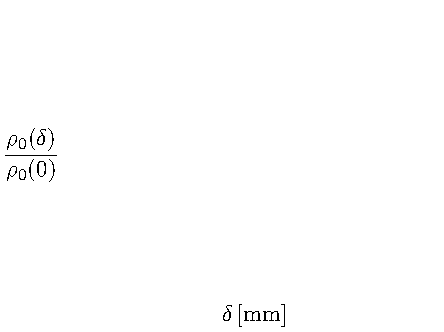
\includegraphics{P1/CeramBobineDDEDPUPSimuExp}} 
\noindent Dans la pratique, nous mesurons en fait le gain en \ddedpup en comparant l'effet d'une céramique avec une déviation d'amplitude $\Devi$ à l'effet de la même céramique sans déviation ($\Devi=0$). En d'autres termes, nous ne mesurons pas :
\[
\GainCeram 
\equiv \frac{\rhojetaxe(\Devi)}{\AvecTexte{\rhojetaxe}{sans céramique}}
\virguleformule
\mbox{ mais }\frac{\rhojetaxe(\Devi)}{\rhojetaxe(0)}
\pointformule
\]
\noindent La figure ci-contre représente les résultats de la simulation numérique pour  $\tfrac{\rhojetaxe(\Devi)}{\rhojetaxe(0)}$ (ligne continue), ainsi que les points mesurés expérimentalement.


\casse


\subsubsection{Influence des autres pièces de céramiques}
Il convient de mentionner que la grandeur physique à laquelle nous avons accès sur notre \setup n'est en fait pas exactement $\ttfrac{\rhojetaxe(\Devi)}{\rhojetaxe(0)}$. En effet, notre guide ne comporte pas qu'une seule pièce de céramique, mais une dizaine, réparties tous les \cm{40} environ. 
Pour notre étude nous utilisons \emph{l'une de ces céramiques}, placée environ \m{1} après l'entrée du guide. Ceci implique en outre que le \jat, au moment où il passe à travers \emph{cette} céramique, est déjà passé à travers d'autres pièces avant et en traversera d'autres après. 

\Resultat
{
Nous avons vu que, dans cette gamme de température ($\approx\microK{600}$), chaque céramique a un effet sur le jet, même si celui-ci n'est pas dévié. 
Nous mesurons donc toujours l'influence de toutes les céramiques, \emph{dont l'une seulement} est en présence d'une déviation d'amplitude $\Devi$ du \jat. 
}

De plus, cela veut dire que le jet est en permanence maintenu légèrement hors d'\eqthdy, puisque chaque céramique tronque partiellement la distribution atomique. Le jet n'a en effet pas le temps de \rether entre deux céramiques successives. La simulation numérique décrite dans la \autoref{sec:CeramSimu}, elle, ne rend pas compte de l'influence de toutes les céramiques puisqu'elle ne fait pas intervenir les processus collisionnels.


\subsection{Gain en \tcolel}\label{sec:CeramSimuGainTcol}
Dans le chapitre~\nref{chap:JetAtomique} nous avons souligné l'importance de maintenir un \tcolel soutenu au sein du jet. La figure~\nref{fig:CeramBobineGammaSimu} représente les résultats de la simulation numérique pour le gain en \tcolel 
$
\ttfrac{\gammacolapres}{\gammacol}
%\virguleformule
$
obtenu après \reth, en considérant comme précédemment $\CeramLong=\micron{10}$, $\CeramLong=\mm{5}$, $\CeramLong=\mm{10}$ et $\CeramLong=\mm{100}$.
%
\bfighs
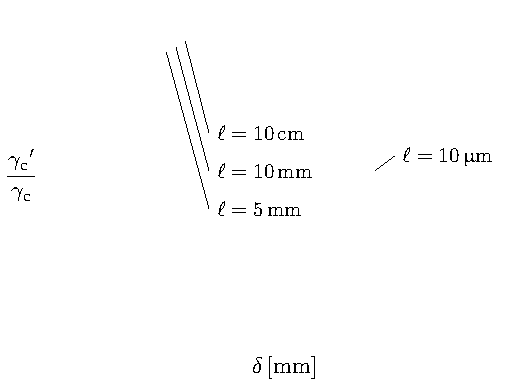
\includegraphics{P1/CeramBobineGammaSimu}
\CaptionFigss{Représentation des résultats de la simulation numérique pour le gain en \tcolel $\ttfrac{\gammacolapres}{\gammacol}$ en fonction de la distance $\Devi$ de déviation. Les différentes courbes correspondent à différentes longueurs de céramique. Le caractère \bd de l'évaporation mentionné en \autoref{sec:CeramBiDimensionnalité} permet d'augmenter substantiellement le \tcolel.
}
\label{fig:CeramBobineGammaSimu}
\efigh

\casse

Nous constatons sur la figure~\nref{fig:CeramBobineGammaSimu} qu'il est possible d'augmenter sensiblement le \tcolel : $6\%$ dans nos conditions expérimentales et jusqu'à $10\%$ pour une évaporation quasi-\bde%
%\footnote
{% 
. Cependant, pour obtenir les gains maximaux mentionnés ci-dessus (respectivement $6\%$ et $10\%$), il faut se contenter alors de gains plus modestes pour la \ddedpup (respectivement $1,3$ et $1,7$ environ)~\cite{LaG06}.
}%
\noindent Notons que les remarques faites sur la figure~\nref{fig:CeramBobineDDEDPUPSimu} (page \pageref{sec:CeramBobineDDEDPUPSimuInterpretation}) sont aussi valables pour la figure~\nref{fig:CeramBobineGammaSimu}.

\Resultat{La déviation du jet au niveau d'une \pdec permet en principe d'augmenter significativement le \tcolel, tout particulièrement si l'élimination est rendu \bde. Rappelons toutefois (voir la \autoref{sec:RethermJet}) que ce point est directement lié au fait que le \ppt n'est pas harmonique.}




\section{Déviation du jet à l'aide d'aimants permanents}\label{sec:EvapCeramAimants}
Nous avons décrit dans la \autoref{sec:EvapCeramMiseEnOeuvre} comment dévier la trajectoire moyenne du \jat à l'aide d'une paire de bobines positionnée symétriquement de part et d'autre du guide. Nous pouvons ainsi contrôler l'amplitude $\Devi$ de la déviation avec une grande précision.
Dans la perspective d'utiliser un grand nombre de zones d'évaporation, ce dispositif souffre cependant de quelques défauts :
\begin{itemize}
	\item l'encombrement spatial des bobines (d'environ \cm{10} suivant l'axe du guide) rend difficile l'enchainement de zones d'évaporation,
	\item la fabrication d'un grand nombre de bobines peut rendre la mise en pratique fastidieuse,
	\item il est nécessaire de disposer d'autant de sources de courant stabilisées que de paires de bobines.
\end{itemize}

Cette section a pour but de présenter brièvement une mise en \oe uvre beaucoup plus compacte de la méthode d'évaporation du jet sur une surface. Celle-ci, se basant sur l'utilisation d'aimants permanents, est bien moins onéreuse et sa mise en \oe uvre est rapide (pas de bobines à fabriquer, pas besoin d'alimentations stabilisées).

\subsection{Mise en \oe uvre}
\Cahier{8,62-65}
Dans cette sous-section nous décrivons brièvement le \setup qui nous permet d'évaporer le \jat sur une céramique à l'aide d'aimants permanents.
Tout comme nous l'avons vu dans la \autoref{sec:EvapCeramBobines}, il est important de produire une configuration antisymétrique de \chm par rapport à l'axe $z$ afin de ne pas produire de colline de potentiel le long du trajet du jet. 

\inlinefig{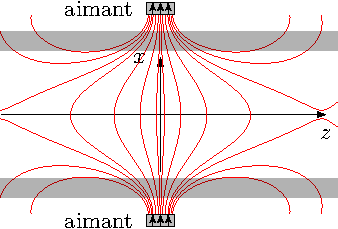
\includegraphics{P1/GuideChampTransMagnets}} 
Les aimants que nous utilisons sont composés d'un alliage de Niobium (Nb-Fe-B). L'annexe~\nref{annexe:ModelisationAimants} précise leurs caractéristiques. Deux aimants sont montés de manière symétrique, de part et d'autre du guide, au niveau de l'une des céramique. Les aimantations sont dirigées dans le même sens, suivant les $x$ croissants dans notre cas. La figure ci-contre représente quelques lignes du \chm ainsi produit dans le plan ($x,z$).
\noindent Afin de contrôler précisément l'écart $\Daimants$ entre les deux aimants, ceux-ci sont fixés sur des platines de micro-positionnement (voir la figure~\nref{fig:EvapMagnet}). 
Nous pouvons ainsi faire varier $\Daimants$ sur une plage de $58$ à $\mm{90}$. 
%La  représente une photographie du montage.
\picskip{0}
%
\bfigh
\RemonteUnPeuFig
{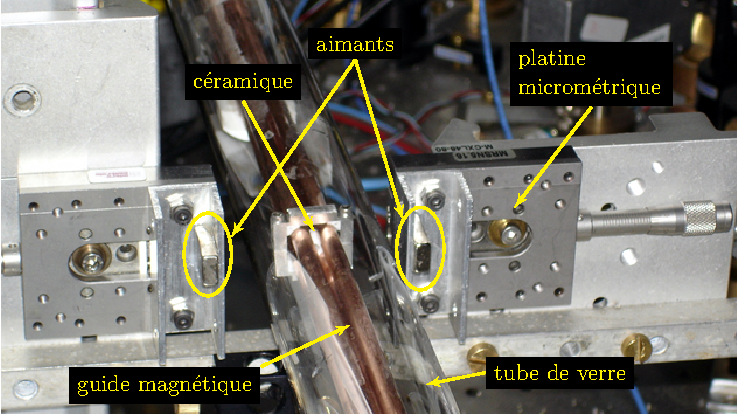
\includegraphics[scale=1]{P1/CeramEvapMagnets}}
\RemonteUnPeuFig
\CaptionFig{
(b) : photographie du \setup permettant d'évaporer le \jat sur une pièce de céramique. On y voit une portion du \gm sur laquelle se trouve l'une des pièces de céramique. De part et d'autre du guide, les deux platines de micro positionnement permettent d'ajuster la distance séparant les aimants de \mm{58} à \mm{90}.
}
\label{fig:EvapMagnet}
\efigh

\ifthenelse{\FormatEUE > 0}{}
{\AjouteLigne}

\subsection{Calibration du \chm produit par les aimants}
Afin de connaître précisément l'amplitude $\Devi$ de la déviation du jet il est impératif de calibrer la valeur du \chm transverse $\CeramBtrans$ imposé par les aimants au voisinage de l'axe $z$ du guide.
Celle-ci dépend naturellement de l'écart $\Daimants$ entre les deux aimants. La figure~\nref{fig:CeramAimantChamp} représente les mesures du \chm transverse 
%prises au long de l'axe $z$ pour différents écart $\Daimants$, ainsi que la valeur maximale $\Btransmax$, au niveau de la pièce de céramique, 
en fonction de $\Daimants$. 
\bfighsss
\subfloat[]{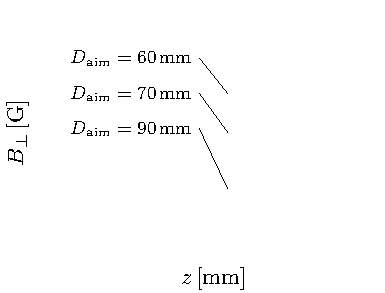
\includegraphics{P1/CeramAimantChampZ}}\,\,\,\,\,\,
\subfloat[]{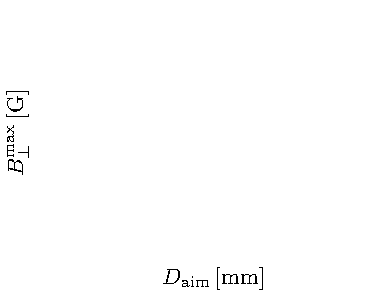
\includegraphics{P1/CeramAimantChampMax}}
\CaptionFigss{
(a) : mesure du \chm transverse $\CeramBtrans$ produit par les aimants en fonction de la position sur l'axe $z$. L'abscisse $z=0$ correspond à la position de la \pdec. Chaque courbe correspond à un écartement $\Daimants$ différent.\\
(b) : mesure du \chm transverse $\Btransmax$ produit au niveau de la \pdec en fonction de l'écart entre les aimants. La valeur $\Btransmax$ donne l'amplitude de la déviation $\Devi$ au niveau de la céramique grâce à la relation \vref{eq:Devi}.}
\label{fig:CeramAimantChamp}
\efigh

%Rappelons que c'est $\Btransmax$ qui donne l'amplitude de la déviation $\Devi$ grâce à la relation \vref{eq:Devi}.

\casse

\subsection{Variation du \fat}\label{sec:ResultatVariationFluxAimants}
Afin de valider cette technique se basant sur l'utilisation d'aimants permanents, nous la comparons brièvement à celle basée sur l'utilisation de bobines. 
Dans cette sous-section, nous présentons donc l'effet de ce dispositif sur le jet en terme de réduction du \fat, comme dans la \autoref{sec:ResultatVariationFlux}. 
La figure \vref{fig:CeramAimantFat} témoigne de l'équivalence de ces deux méthodes.
\bfighs
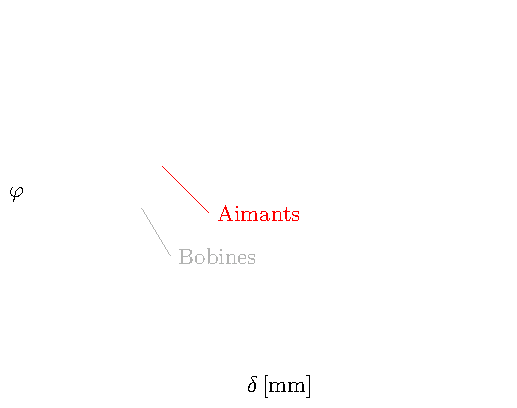
\includegraphics{P1/CeramAimantFat}
\CaptionFigss{Comparaison entre l'utilisation de bobines et l'utilisation d'aimants permanents. Nous représentons la réduction relative de \fat $\rapflux\equiv\ttfrac{\flux(\Devi)}{\flux(0)}$ des flux traversant la pièce en céramique avec, et sans déviation, en fonction de l'amplitude $\Devi$ de la déviation. \\
Les carrés grisés représentent les données de la figure \vref{fig:CeramBobineFat} (utilisation de bobines). \\
Les ronds rouges correspondent aux mesures effectuées en déviant la trajectoire à l'aide d'aimants permanents. Le \fat sans déviation est mesuré en retirant le dispositif représenté sur la figure~\nref{fig:EvapMagnet}.
Les valeurs négatives de $\Devi$ se rapportent à une déviation dans l'autre sens et sont obtenues en inversant l'orientation du dispositif.}
\label{fig:CeramAimantFat}
\efigh

\RemonteUnPeuFig
\RemonteUnPeuFig

\section{Conclusion}
Dans ce chapitre, nous avons présenté une technique permettant de mener à bien l'\evap d'un \jatmg. Nous avons adapté le principe d'élimination d'atomes énergétiques au contact d'une surface matérielle~\cite{HMO03} à notre \setup. Pour cela nous dévions localement la trajectoire du jet vers l'une des \pdecs présente dans notre \gm. 

\noindent Le contrôle de la déviation est assuré par la superposition local d'un \chm $\CeramBtrans$ transverse à l'axe du guide. 
Deux techniques sont présentées afin de produire ce champ:
\begin{itemizel}
	\item l'une se basant sur l'utilisation de bobines, 
	\item l'autre à base d'aimants permanents.
\end{itemizel}


%\casse

Ce processus d'évaporation peut, dans certaines conditions, être aisément rendu bidimensionnel et présente plusieurs avantages majeurs en comparaison de l'évaporation par \firf décrit dans le chapitre~\nref{chap:JetAtomique}:
\begin{itemizel}
	\item l'efficacité de l'élimination des atomes répondant au critère de filtrage est de $100\%$,
	\item l'action de \fisp est beaucoup plus locale puisqu'elle se produit au contact de la surface, soit quelques millimètres de long dans notre cas.
\end{itemizel}



%\subsubsection{Ouverture, possibilité de miniaturisation}
Concluons ce chapitre en soulignant un dernier point relatif à cette technique. Jusqu'ici nous avons décrit le cas d'un jet dévié de l'axe $z$ du \gm afin de lui faire approcher la surface d'une \pdec. 
\inlinefig{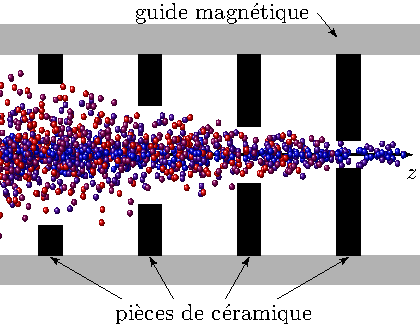
\includegraphics{P1/CeramPetitPetit}} 
Essayons d'imaginer un \setup qui serait optimisé pour pouvoir utiliser au mieux cette technique d'évaporation. Nous pourrions par exemple envisager de ne plus dévier le jet de son axe, mais plutôt d'utiliser tout au long du guide des céramiques dont le trou central serait de plus en plus étroits au fur et à mesure de la propagation. L'illustration ci-contre schématise cette idée en représentant un \jat se propageant suivant l'axe $z$ et passant à travers quatre \pdecs. Chacune d'elles élimine des atomes dont l'énergie est de plus en plus faible. 
\picskip{0}
Cet agencement, qui possède une symétrie de révolution, présente l'énorme avantage de produire une \emph{évaporation strictement \bde}, quelles que soient les conditions de piégeage et de température du jet. 
Sur un plan purement technique en revanche, ce type de dispositif est \emph{très peu flexible} puisqu'une fois placé dans un environnement \uv, il serait difficile d'ajuster la géométrie du système. L'espacement et les diamètres des céramiques devraient alors être calculés à l'avance, pour des caractéristiques initiales du jet très précises (en termes de flux, température, vitesse moyenne, confinement). 

\ifthenelse{\FormatEUE > 0}{}
{\AjouteLigne}

Pour prolonger cette idée, pourquoi ne pas envisager l'optimisation et la miniaturisation de ce type de structure? 
La figure~\nref{fig:CeramContinue} illustre l'utilisation d'une unique surface à symétrie de révolution dont la forme serait optimisée pour mener à bien le \rpef d'un \jatmg. L'encombrement total du système serait fonction uniquement des caractéristiques du jet incident, et non plus des contraintes liées à la portée d'une antenne \rf ou encore à l'encombrement de bobines. 
%Cette idée est à mettre en regard d'expériences effectuées dans le groupe d'Eric Cornell (\nomofficiel{University of Colorado}), et qui consistent à guider des atomes à l'intérieur de fibres optiques creuses~\cite{RMV95,MCA00}.
\bfighs
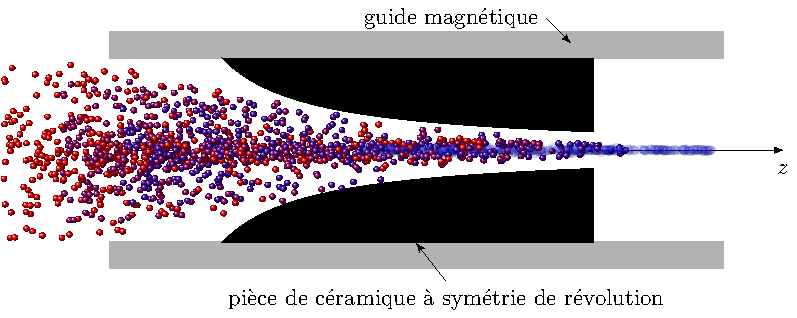
\includegraphics{P1/CeramContinue}
\CaptionFigss{Illustration d'une idée de principe. Une unique surface à symétrie de révolution à l'intérieur de laquelle peut se propager un \jatmg. La forme de cette surface serait optimisée afin de refroidir un jet ayant des caractéristiques données. Si ces dernières le permettent, la surface pourrait même être vue comme un système \sotosay{compact} acceptant un jet thermique \sotosay{en entrée} et fournissant \sotosay{en sortie} un faisceau de matière dans le \rdq.}
\label{fig:CeramContinue}
\efigh



